\documentclass[%
%10pt,
%varwidth=false,
%crop=true,
border={0mm 0mm 0mm 0mm}]{standalone}
\usepackage[T1]{fontenc}
\usepackage[utf8]{inputenc}
\usepackage[auto]{microtype}
%\usepackage{cmbright}
\usepackage{arev}
\usepackage{amsmath, amssymb, amsfonts, icomma}
\usepackage[version=4]{mhchem}
\usepackage{tikz}
\usetikzlibrary{positioning}
\usepackage{chemplants-tub}
\usepackage{xcolor}
%define stream tip, default is stealth
\setchpstreamtip{latex}
\setchpmainstreamthickness{thick}
%\setchpunitthickness{very thick}

\pgfdeclarelayer{bg}    % declare background layer
\pgfsetlayers{bg,main}  % set the order of the layers (main is the standard layer)

\definecolor{signalgruen}{RGB}{49,127,67}    % RAL 6032 Wasser
\definecolor{signalrot}{RGB}{155,36,35}      % RAL 3001 Dampf
\definecolor{signalgrau}{RGB}{150,153,146}   % RAL 7004 Luft
\definecolor{signalgelb}{RGB}{229,190,001}   % RAL 1003 brennbare und nicht brennbare Gase
\definecolor{signalorange}{RGB}{208,93,40}   % RAL 2010 Säuren
\definecolor{signalviolett}{RGB}{132,76,130} % RAL 4008 Laugen
\definecolor{signalbraun}{RGB}{121,77,62}    % RAL 8002 brennbare und nicht brennbare Flüssigkeiten
\definecolor{signalblau}{RGB}{30,45,110}     % RAL 5005 Sauerstoff

% TABLEAU-10
\definecolor{Tab10-A}{RGB}{78, 121, 167}
\definecolor{Tab10-B}{RGB}{242, 142, 43}
\definecolor{Tab10-C}{RGB}{225, 87, 89}
\definecolor{Tab10-D}{RGB}{118, 183, 178}
\definecolor{Tab10-E}{RGB}{89, 161, 79}
\definecolor{Tab10-F}{RGB}{237, 201, 72}
\definecolor{Tab10-G}{RGB}{176, 122, 161}
\definecolor{Tab10-H}{RGB}{255, 157, 167}
\definecolor{Tab10-I}{RGB}{156, 117, 95}
\definecolor{Tab10-J}{RGB}{186, 176, 172}

\begin{document}
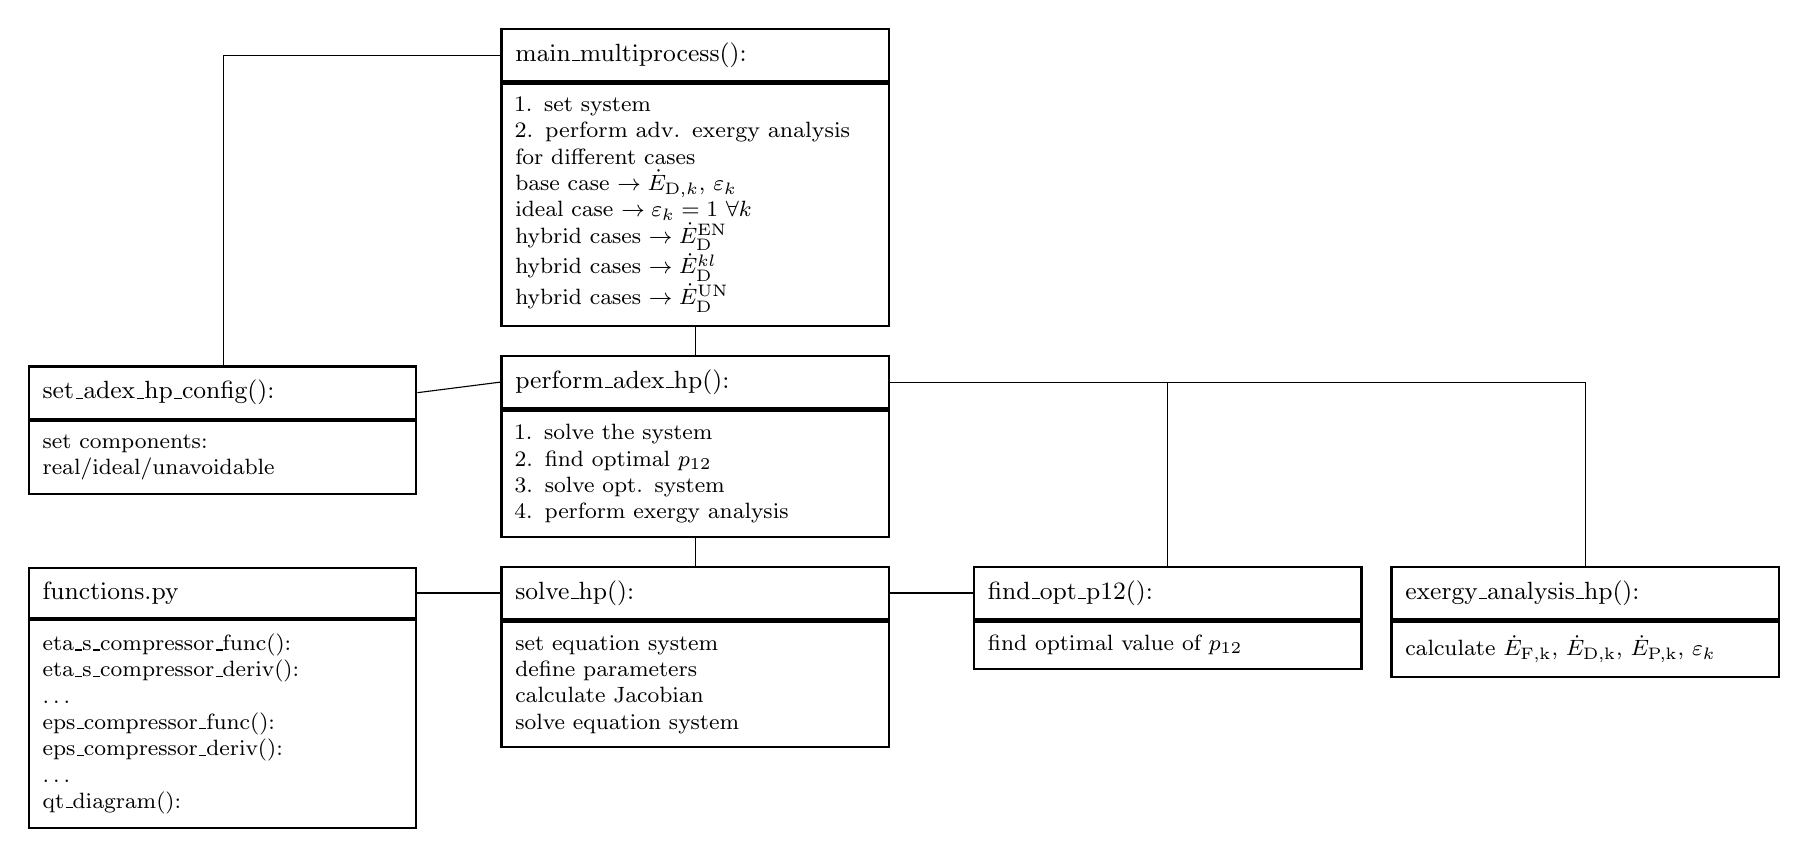
\begin{tikzpicture}[font=\footnotesize] 
%

%help grid and labels
%\draw[help lines] (-2,-3) grid (15,5);
%\foreach \pos in {-2,-1,0,1,2,3,4,5,6,7,8,9,10,11,12,13,14,15}
%\draw[shift={(\pos,-3)}] (0pt,2pt) -- (0pt,-2pt) node[below] {$\pos$};
%\foreach \pos in {-3,-2,-1,0,1,2,3,4,5}
%\draw[shift={(-2,\pos)}] (2pt,0pt) -- (-2pt,0pt) node[left] {$\pos$};

%%% nodes and boxes

%%% NETWORK
\node [rectangle, draw=black, minimum width=140pt, text width= 130pt, thick, inner sep=5pt, align=left] (main) at (1,4) {\small main\_multiprocess():};
\node [rectangle, draw=black, minimum width=140pt, text width= 130pt, thick, inner sep=5pt, align=left, anchor=north] (main-sub) at (main.south) {1. set system \\
2. perform adv. exergy analysis for different cases \\ base case $\rightarrow \dot{E}_{\text{D},k},\ \varepsilon_k$\\ ideal case $\rightarrow \varepsilon_k=1\ \forall k$\\ hybrid cases $\rightarrow \dot{E}_\text{D}^{\text{EN}}$\\ hybrid cases $\rightarrow \dot{E}_\text{D}^{kl}$\\ hybrid cases $\rightarrow \dot{E}_\text{D}^{\text{UN}}$};

%%% SET CONFIG
\node [rectangle, draw=black, minimum width=140pt, text width=130pt, thick, inner sep=5pt, align=left, left=30pt of main, shift={(0, -122pt)}] (set) {\small set\_adex\_hp\_config():};
\node [rectangle, draw=black, minimum width=140pt, text width= 130pt, thick, inner sep=5pt, align=left, anchor=north] (set-sub) at (set.south) {set components: \\ real/ideal/unavoidable};



%%% PERFORM ADEX
\node [rectangle, draw=black, minimum width=140pt, text width= 130pt, thick, inner sep=5pt, align=left, below = 10pt of main-sub] (perform-adex) {\small perform\_adex\_hp():};
\node [rectangle, draw=black, minimum width=140pt, text width= 130pt, thick, inner sep=5pt, align=left, anchor=north] (perform-adex-sub) at (perform-adex.south) {1. solve the system \\ 2. find optimal $p_{12}$ \\ 3. solve opt. system\\ 4. perform exergy analysis};

%%% SOLVE
\node [rectangle, draw=black, minimum width=140pt, text width= 130pt, thick, inner sep=5pt, align=left, below=10pt of perform-adex-sub] (solve) {\small solve\_hp():};
\node [rectangle, draw=black, minimum width=140pt, text width= 130pt, thick, inner sep=5pt, align=left, anchor=north] (solve-sub) at (solve.south) {set equation system \\ define parameters \\ calculate Jacobian \\ solve equation system};

%%% FIND OPT P12
\node [rectangle, draw=black, minimum width=140pt, text width= 130pt, thick, inner sep=5pt, align=left, right=30pt of solve] (opt) {\small find\_opt\_p12():};
\node [rectangle, draw=black, minimum width=140pt, text width= 130pt, thick, inner sep=5pt, align=left, anchor=north] (opt-sub) at (opt.south) {find optimal value of $p_{12}$};

%%% EXERGY ANALYSIS
\node [rectangle, draw=black, minimum width=140pt, text width= 130pt, thick, inner sep=5pt, align=left, right=10pt of opt] (exergy) {\small exergy\_analysis\_hp():};
\node [rectangle, draw=black, minimum width=140pt, text width= 130pt, thick, inner sep=5pt, align=left, anchor=north] (exergy-sub) at (exergy.south) {calculate $\dot{E}_{\text{F,k}},\ \dot{E}_{\text{D,k}},\ \dot{E}_{\text{P,k}},\ \varepsilon_k$};

%%% FUNCTIONS
\node [rectangle, draw=black, minimum width=140pt, text width= 130pt, thick, inner sep=5pt, align=left, left=30pt of solve] (functions) {\small functions.py};
\node [rectangle, draw=black, minimum width=140pt, text width= 130pt, thick, inner sep=5pt, align=left, anchor=north] (fluids-sub) at (functions.south) {eta\_s\_compressor\_func(): \\ eta\_s\_compressor\_deriv(): \\ \ldots \\ eps\_compressor\_func(): \\ eps\_compressor\_deriv():\\ \ldots \\ qt\_diagram():};


%%% connections, arrows

\draw [solid] (perform-adex-sub.south) -- (solve.north);
\draw [solid] (exergy.north) -- ++(0,0) |- (perform-adex.east);
\draw [solid] (main.west) -- ++(-100pt,0) |- (set.north);
\draw [solid] (solve.east) -- ++(15pt,0) |- (opt.west);
\draw [solid] (main-sub.south) -- (perform-adex.north);
\draw [solid] (set.east) -- (perform-adex.west);
\draw [solid] (opt.north) -- ++(0,0) |- (perform-adex.east);

\draw [solid] (solve.west) -- (functions.east);

\end{tikzpicture}

\end{document}